\section{Protocols}

\secttoc

The following abbreviations are used:

\begin{description}
  \item[OPeer] An Ordinary Peer
  \item[SPeer] A Super Peer
  \item[Req.] Send a request message
\end{description}

\subsection{Joining the network}

This involves contacting the Host Cache for the IDs of Super Peers, and
requesting a connection.  The connection can either be accepted or denied. If
the connection is accepted, the peer sends their list of shared files to the
connected Super Peer.

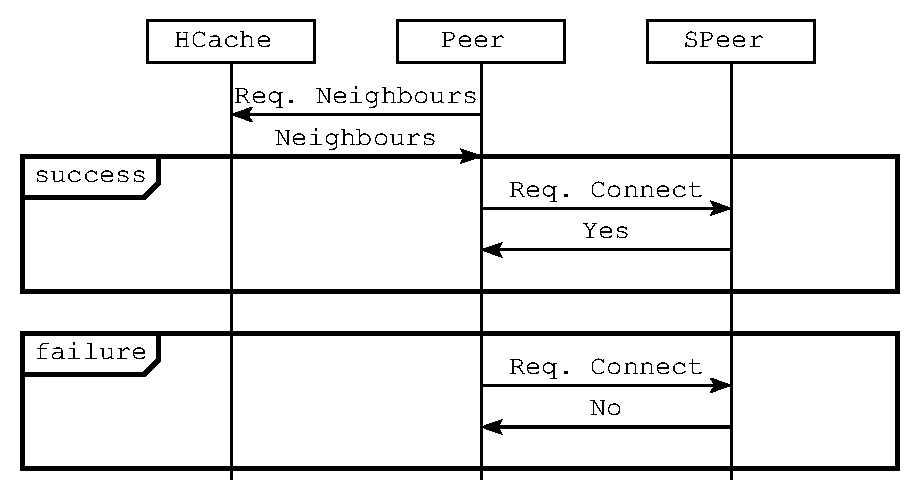
\includegraphics{protocol_connect.eps}

\subsection{Send file-list}

Only ordinary Peers send a file list.

\includegraphics{protocol_send_file_list.eps}

\subsection{Searching for Files}

In the following example, there are only two Super Peers in the network.  The
search request is forwarded throughout the network, and if at some point a Super
Peer is able to locate it, the location is passed back through the network to
the original requester.

\includegraphics{protocol_file_search.eps}

\subsection{Acquiring Files}

Once a file location has been determined, acquiring it is straightforward direct
communication between two peers.

\includegraphics{protocol_acquire_file.eps}
